\chapter{OpenGL}
\todo{This Chapter describes OpenGL and which of its functionalities we have used to create our game.}

\section{Analysis}

\section{Design}
Firstly \ref{fig:terminology} shows how we represent abstract class names and how we denote public or private attributes and methods.\todo{Skal det stå her? Det må være C\# UML standard det her.}
\begin{figure}[H]
\centering
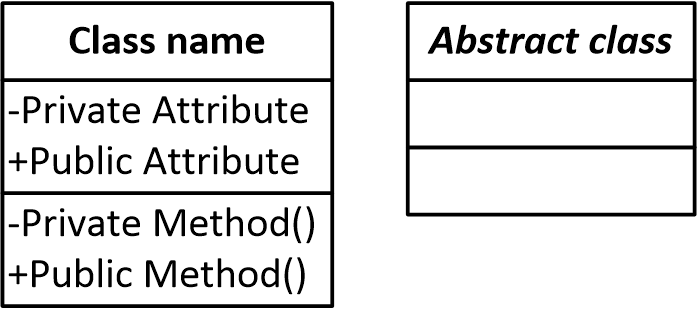
\includegraphics[width=0.4\linewidth]{img/terminology.png}%0.1 margin
\caption{The way we make UML described in a figure.}
\label{fig:terminology}
\end{figure}


\begin{figure}[H]
\centering
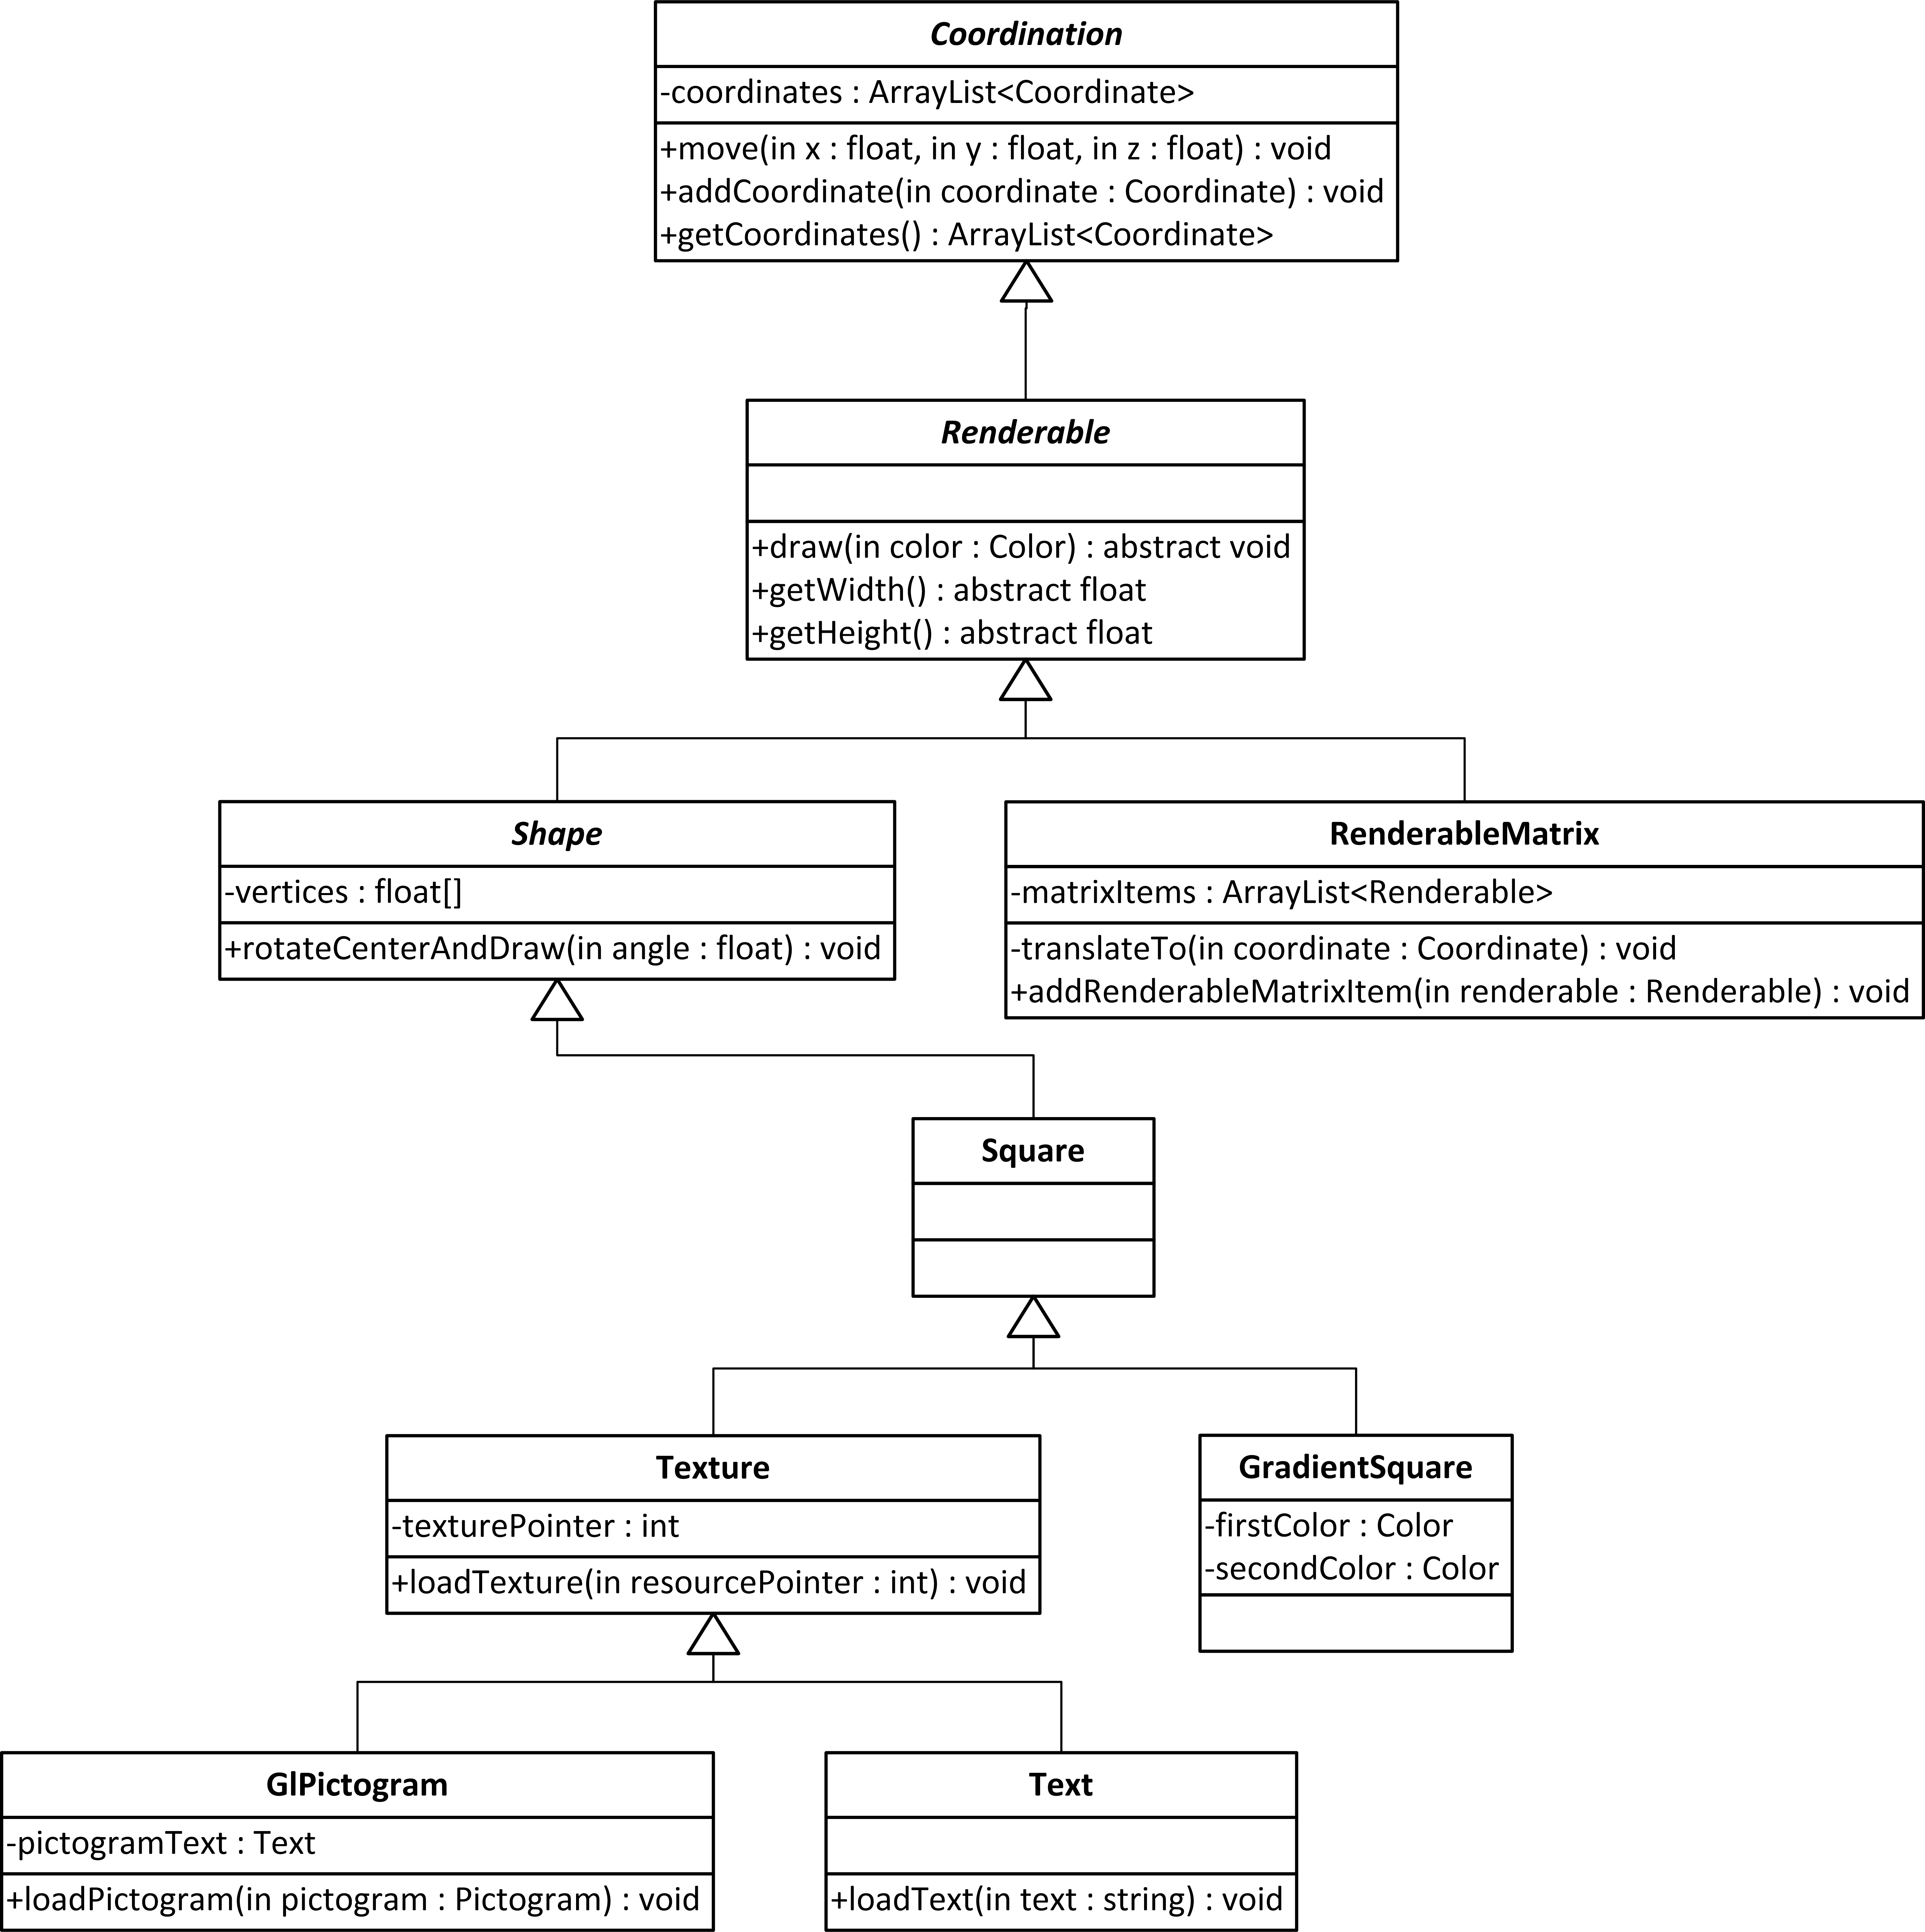
\includegraphics[width=0.9\linewidth]{img/renderables.png}%0.1 margin
\caption{Class diagram of the objects that can be rendered.}
\label{fig:renderables}
\end{figure}


\begin{figure}[H]
\centering
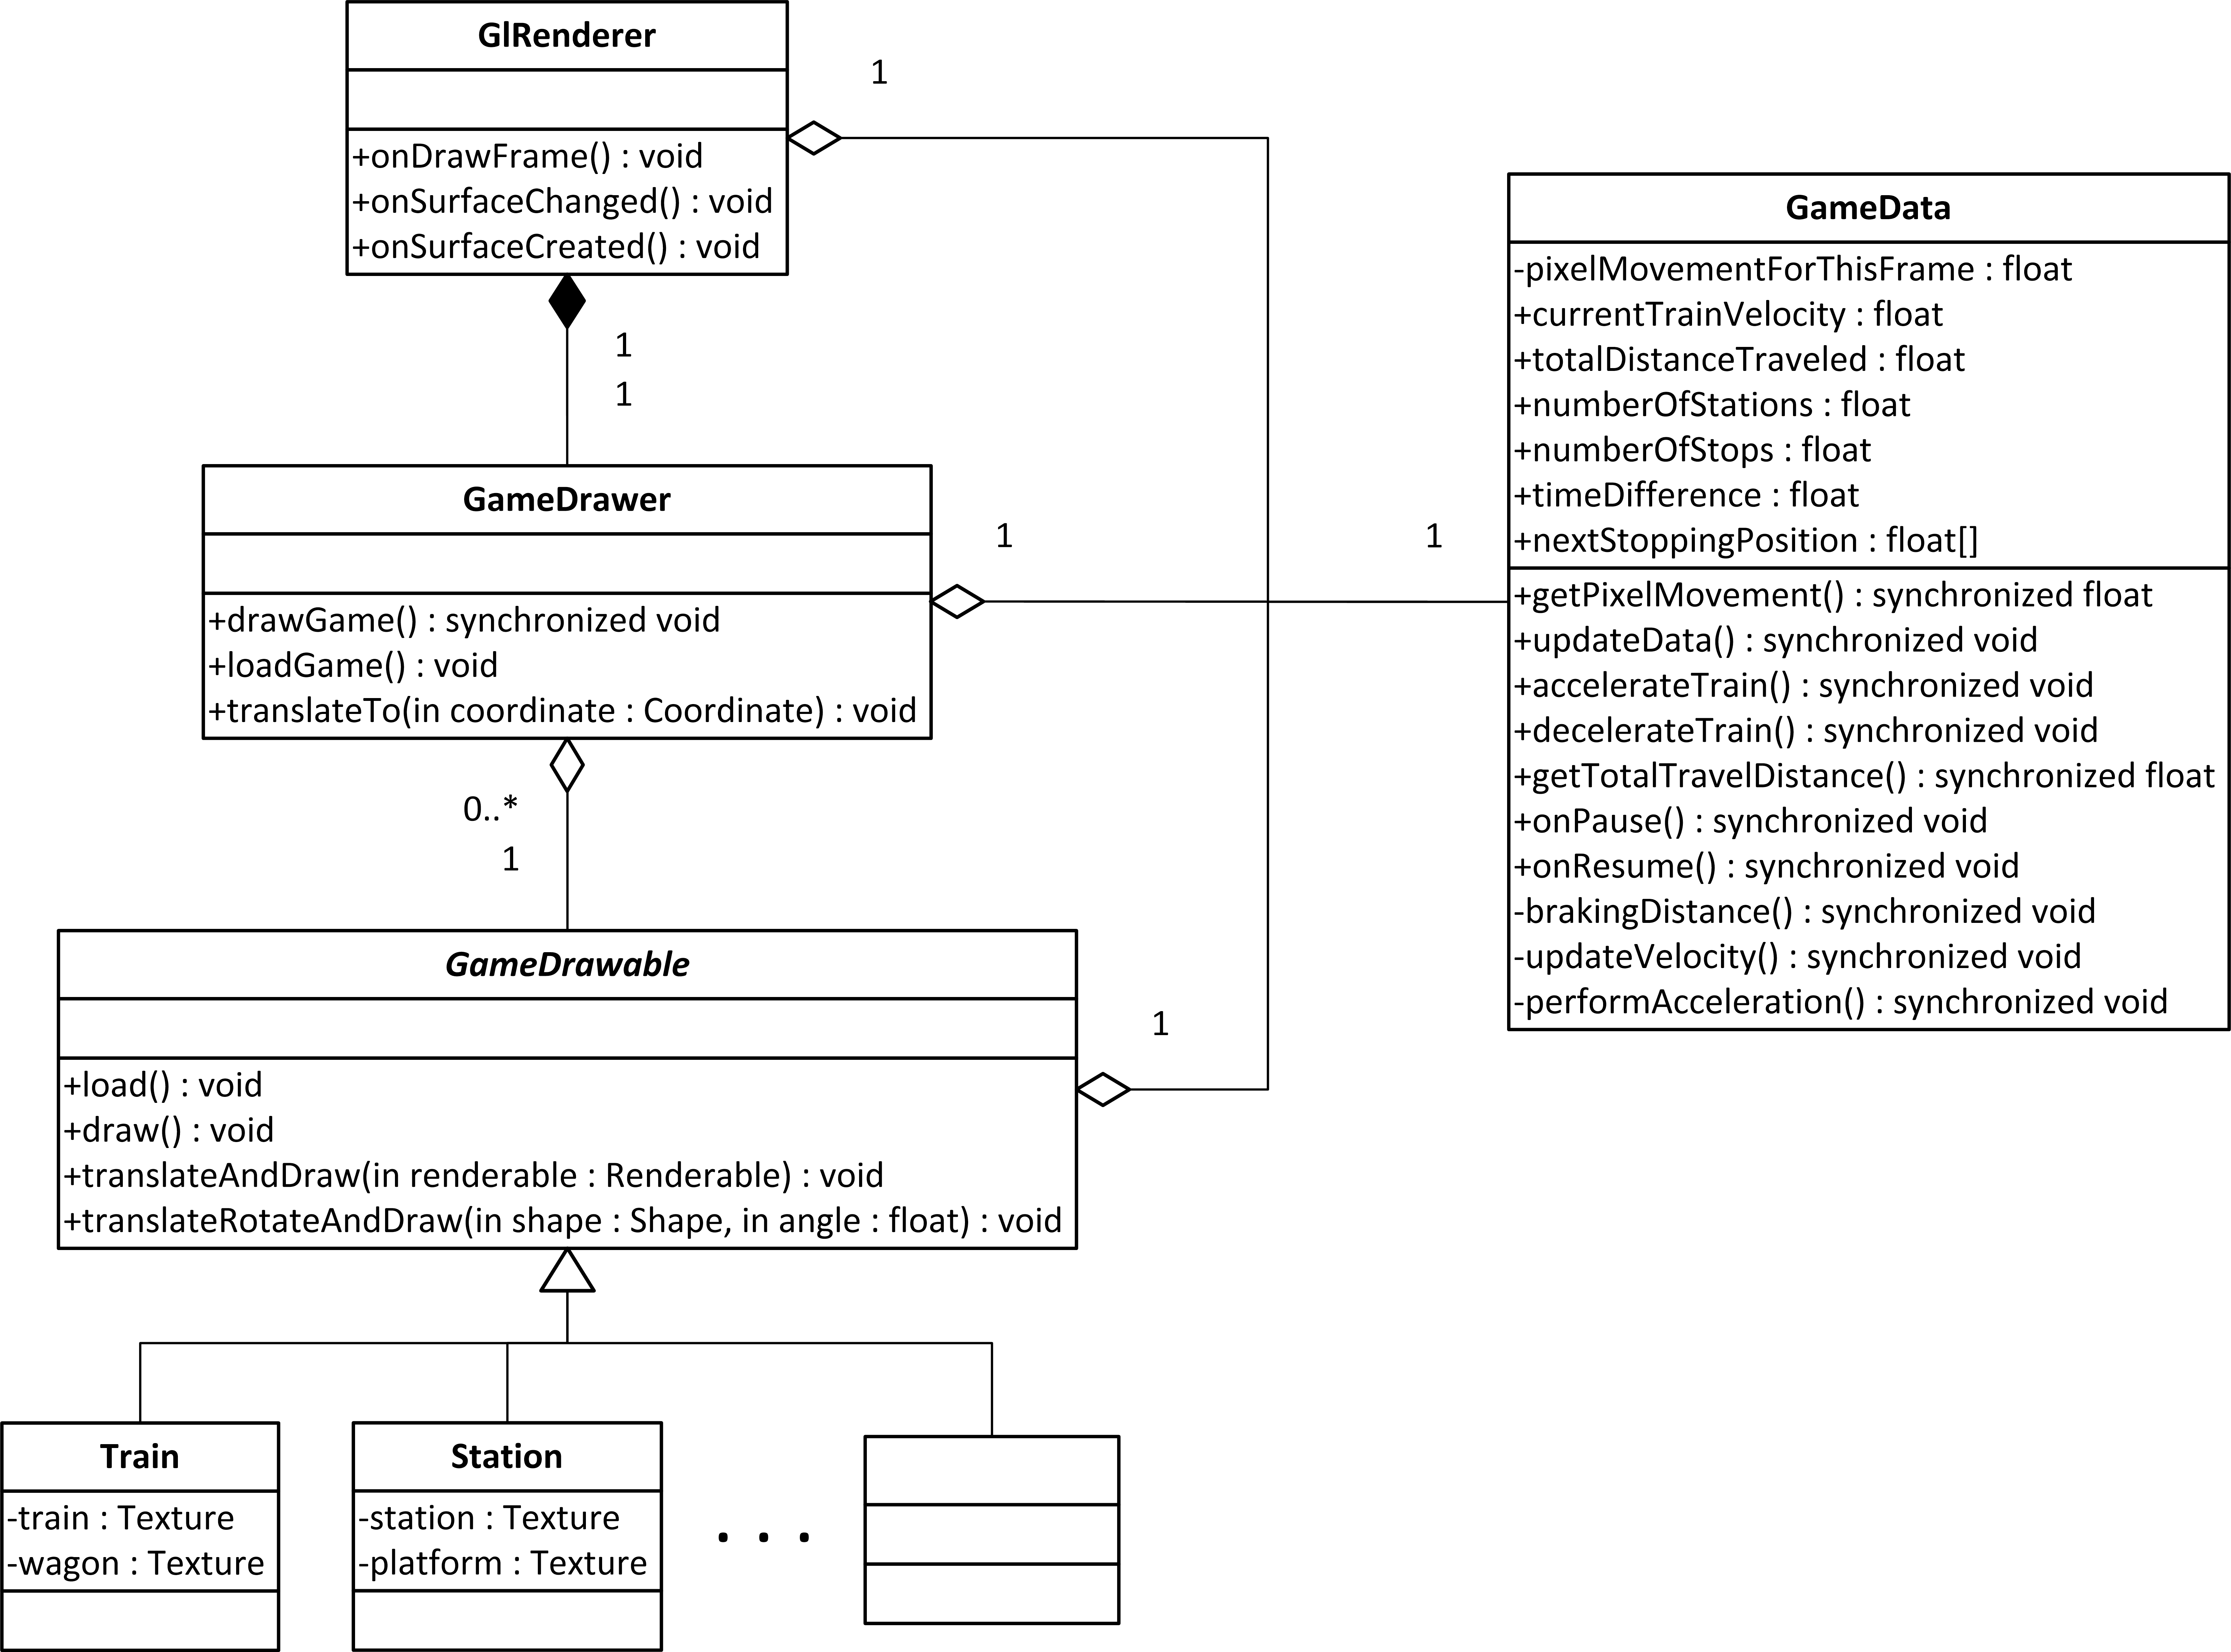
\includegraphics[width=0.9\linewidth]{img/game.png}%0.1 margin
\caption{Class diagram of the objects involved with drawing the game.}
\label{fig:game}
\end{figure}

\section{Implementation}

\todo{Describes the implementation of OpenGL}